% !TeX root = RJwrapper.tex
\title{spinifex: An R Package for Creating a Manual Tour of Low-dimensional
Projections of Multivariate Data}
\author{by Nicholas Spyrison, Dianne Cook}

\maketitle

\abstract{%
Dynamic low-dimensional linear projections of multivariate data
collectively known as \emph{tours} provide an important tool for
exploring multivariate data and models. The R package \pkg{tourr}
provides functions for several types of tours: grand, guided, little,
local and frozen. Each of these can be viewed dynamically, or saved into
a data object for animation. This paper describes a new package,
\pkg{spinifex}, which provides a manual tour of multivariate data where
the projection coefficient of a single variable is controlled. The
variable is rotated fully into the projection, or completely out of the
projection. The resulting sequence of projections can be displayed as an
animation, with functions from either the \pkg{plotly} or
\pkg{gganimate} packages. By varying the coefficient of a single
variable, it is possible to explore the sensitivity of structure in the
projection to that variable. This is particularly useful when used with
a projection pursuit guided tour to simplify and understand the
solution. The use of the manual tour is applied particle physics data to
illustrate the sensitivity of structure in a projection to specific
variable contributions.
}

\hypertarget{introduction}{%
\section{Introduction}\label{introduction}}

Exploring multivariate spaces is a challenging task, increasingly so as
dimensionality increases. Traditionally, static low-dimensional
projections are used to display multivariate data in two dimensions
including principal component analysis, linear discriminant spaces or
projection pursuit. These are useful for finding relationships between
multiple variables, but they are limited because they show only a
glimpse of the high-dimensional space. An alternative approach is to use
a tour \citep{asimov_grand_1985} of dynamic linear projections to look
at many different low-dimensional projections. Tours can be considered
to extend the dimensionality of visualization, which is important as
data and models exist in more than 3D. The package \CRANpkg{tourr}
\citep{wickham_tourr:_2011} provides a platform for generating tours. It
can produce a variety of tours, each paired with a variety of possible
displays. A user can make a grand, guided, little, local or frozen tour,
and display the resulting projected data as a scatterplot, density plot,
histogram, or even as Chernoff faces if the projection dimension is more
than 3.

This work adds a manual tour to the collection. The manual tour was
described in \citet{cook_manual_1997} and allows a user to control the
projection coefficients of a selected variable in a 2D projection. The
manipulation of these coefficients allows the analyst to explore their
sensitivity to the structure within the projection. As manual tours
operate on only one variable at a time, they are particularly useful
once a feature of interest has been identified.

One way to identify ``interesting'' features is with the use of a guided
tour \citep{cook_grand_1995}. Guided tours select a very specific path,
which approaches a projection that optimizes an objective function. The
optimization used to guide the tour is simulated annealing
\citep{kirkpatrick_optimization_1983}. The direct optimization of a
function allows guided tours to rapidly identify interesting projection
features given the relatively large parameter-space. After a projection
of interest is identified, an analyst can then use the ``finer brush''
of the manual tour to control the contributions of individual variables
to explore the sensitivity they have on the structure visible in the
projection.

The paper is organized as follows. Section \ref{sec:algorithm} describes
the algorithm used to perform a radial manual tour as implemented in the
package \CRANpkg{spinifex}. Section \ref{sec:display} explains how to
generate an animation of the manual tour using the animation frameworks
offered by \CRANpkg{plotly} \citep{sievert_interactive_2020} and
\CRANpkg{gganimate} \citep{pedersen_gganimate_2020}. Package
functionality and code usage following the order applied in the
algorithm follows in section \ref{sec:usage}. Section
\ref{sec:application} illustrates how this can be used for sensitivity
analysis applied to multivariate data collected on high energy physics
experiments \citep{wang_mapping_2018}. Section \ref{sec:discussion}
summarizes this paper and discusses potential future directions.

\hypertarget{sec:algorithm}{%
\section{Algorithm}\label{sec:algorithm}}

The algorithm to conduct a manual tour interactively, by recording
mouse/cursor motion, is described in detail in \citet{cook_manual_1997}.
Movement can be in any direction and magnitude, but it can also be
constrained in several ways:

\begin{itemize}
\tightlist
\item
  \emph{radial}: fix the direction of contribution, and allow the
  magnitude to change.
\item
  \emph{angular}: fix the magnitude, and allow the angle or direction of
  the contribution to vary.
\item
  \emph{horizontal}, \emph{vertical}: allow rotation only around the
  horizontal or vertical axis of the current 2D projection.
\end{itemize}

The algorithm described here produces a \textbf{radial} tour as an
\emph{animation sequence}. It takes the current contribution of the
chosen variable, and using rotation brings this variable fully into the
projection, completely removes it, and then returns to the original
position.

\hypertarget{notation}{%
\subsection{Notation}\label{notation}}

The notation used to describe the algorithm for a 2D radial manual tour
is as follows:

\begin{itemize}
\tightlist
\item
  \(\textbf{X}\), the data, an \(n \times p\) numeric matrix to be
  projected to 2D.
\item
  \(\textbf{B} = (B_1,~ B_2)\), any 2D orthonormal projection basis,
  \(p \times 2\) matrix, describing the projection from
  \(\mathbb{R}^p \Rightarrow \mathbb{R}^2\). This is called this the
  ``original projection'' because it is the starting point for the
  manual tour.
\item
  \(k\), is the index of the variable to manipulate, called the ``manip
  var''. 
\item
  \(\textbf{e}\), a 1D basis vector of length \(p\), with 1 in the
  \(k\)-th position and 0 elsewhere.
\item
  \(\textbf{M}\) is a \(p \times 3\) matrix, defining the 3D subspace
  where data rotation occurs and is called the manip(ulation) space.
\item
  \(\textbf{R}\), the 3D rotation matrix, for performing unconstrained
  3D rotations within the manip space, \(\textbf{M}\).
\item
  \(\theta\), the angle of in-projection rotation, for example, on the
  reference axes; \(c_\theta, s_\theta\) are its cosine and sine.
\item
  \(\phi\), the angle of out-of-projection rotation, into the manip
  space; \(c_\phi, s_\phi\) are its cosine and sine. The initial value
  for animation purposes is \(\phi_1\).
\item
  \(\textbf{U}\), the axis of rotation for out-of-projection rotation
  orthogonal to \(\textbf{e}\).
\item
  \(\textbf{Y}\), the resulting projection of the data through the manip
  space, \(\textbf{M}\), and rotation matrix, \(\textbf{R}\).
\end{itemize}

The algorithm operates entirely on projection bases and incorporates the
data only when making the projected data plots, in light of efficiency.

\hypertarget{steps}{%
\subsection{Steps}\label{steps}}

\hypertarget{step-0-set-up}{%
\subsubsection{Step 0) Set up}\label{step-0-set-up}}

The flea data (\citet{lubischew_use_1962}), available in the \pkg{tourr}
package, is used to illustrate the algorithm. The data contains 74
observations on 6 variables, which are physical measurements made on
flea beetles. Each observation belongs to one of three species.

An initial 2D projection basis must be provided. A suggested way to
start is to identify an interesting projection using a projection
pursuit guided tour. Here the holes index is used to find a 2D
projection of the flea data, which shows three separated species groups.
Figure \ref{fig:step0} shows the initial projection of the data. The
left panel displays the projection basis (\(\textbf{B}\)) and can be
used as a visual guide of the magnitude and direction that each variable
contributes to the projection. The right panel shows the projected data,
\(\textbf{Y}_{[n,~2]} ~=~ \textbf{X}_{[n,~p]} \textbf{B}_{[p,~2]}\). The
color and shape of points are mapped to the flea species. This plot is
made using the \code{view\_basis()} function in \pkg{spinifex}, which
generates a \CRANpkg{ggplot2} \citep{wickham_ggplot2_2016} object.

\begin{Schunk}
\begin{figure}

{\centering 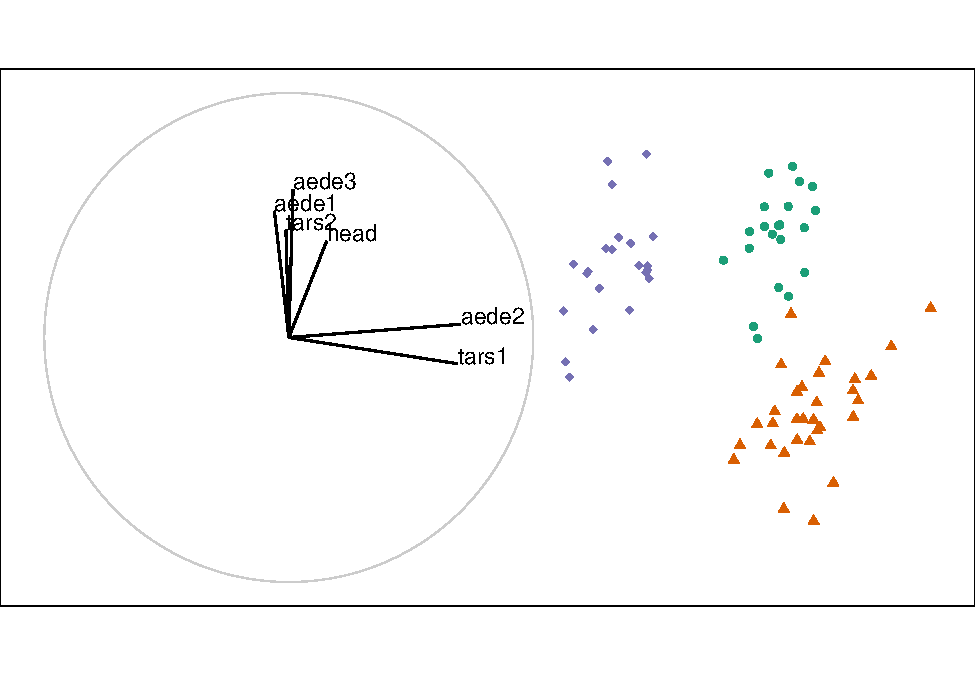
\includegraphics[width=0.7\linewidth]{spyrison-cook_files/figure-latex/step0-1} 

}

\caption[Initial 2D projection]{Initial 2D projection: representation of the basis (left) and resulting data projection (right) of standardized flea data. The color and shape of data points are mapped to beetle species. The basis was identified using a projection pursuit guided tour, with the holes index. The contribution of the variables aede2 and tars1 approximately contrasts the other variables. The visible structure in the projection are the three clusters corresponding to the three species. Produced with the function \code{view\_basis()}.}\label{fig:step0}
\end{figure}
\end{Schunk}

\hypertarget{step-1-choose-manip-variable}{%
\subsubsection{Step 1) Choose manip
variable}\label{step-1-choose-manip-variable}}

In figure \ref{fig:step0} the contribution of the variables tars1 and
aede2 mostly contrast the contribution of the other four variables.
These two variables combined contribute in the direction of the
projection where the purple cluster is separated from the other two
clusters. The variable aede2 is selected as the manip var, the variable
to be controlled in the tour. The question that will be explored is: how
important is this variable to the separation of the clusters in this
projection?

\hypertarget{step-2-create-the-3d-manip-space}{%
\subsubsection{Step 2) Create the 3D manip
space}\label{step-2-create-the-3d-manip-space}}

Initialize the coordinate basis vector as a zero vector, \(\textbf{e}\),
of length \(p\), and set the \(k\)-th element to 1. In the example data,
aede2 is the fifth variable in the data, so \(k=5\), set \(e_5=1\). Use
a Gram-Schmidt process to orthonormalize the coordinate basis vector on
the original 2D projection to describe a 3D manip space, \(\textbf{M}\).

\begin{align*}
  e_k &\leftarrow 1 \\ 
  \textbf{e}^*_{[p,~1]} &= \textbf{e} - \langle \textbf{e}, \textbf{B}_1 \rangle \textbf{B}_1 - \langle \textbf{e}, \textbf{B}_2 \rangle \textbf{B}_2 \\ 
  \textbf{M}_{[p,~3]} &= (\textbf{B}_1,\textbf{B}_2,\textbf{e}^*)
\end{align*}

The manip space provides a 3D projection from \(p\)-dimensional space,
where the coefficient of the manip var can range completely between
{[}0, 1{]}. This 3D space serves as the medium to rotate the projection
basis relative to the selected manipulation variable. Figure
\ref{fig:step2} illustrates this 3D manip space with the manip var
highlighted. This representation is produced by calling the
\code{view\_manip\_space()} function. This diagram is purely used to
help explain the algorithm.

\begin{Schunk}
\begin{figure}

{\centering 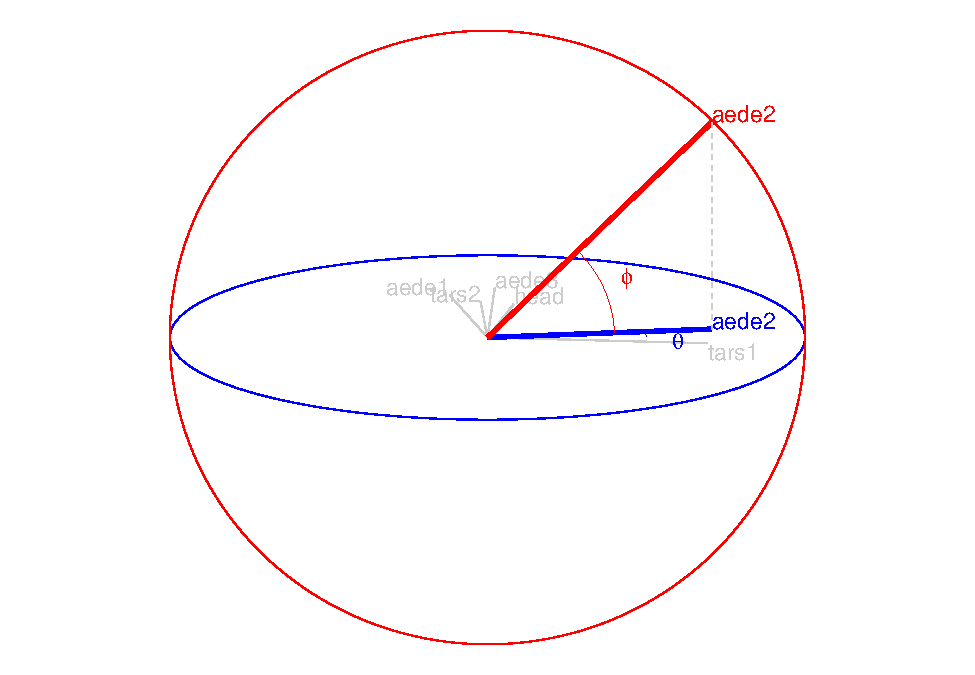
\includegraphics[width=0.7\linewidth]{spyrison-cook_files/figure-latex/step2-1} 

}

\caption[Illustration of a 3D manip space, this space is rotated effectively changing the contribution of the manip variable, aede2 in the example data]{Illustration of a 3D manip space, this space is rotated effectively changing the contribution of the manip variable, aede2 in the example data. The blue circle and variable map lies on the projection plane. The red circle, orthogonal to the projection plane, illustrates the manipulation space and how the manip var can be controlled and how this affects the variable contribution back onto the projection plane. The other variables are omitted from the manipulation dimension for simplicity. Picturing the other variables in that dimension reveals the intuition that rotating one variable performs a constrained rotation on the others. This is illustrated with the \code{view\_manip\_space()} function.}\label{fig:step2}
\end{figure}
\end{Schunk}

\hypertarget{step-3-defining-a-3d-rotation}{%
\subsubsection{Step 3) Defining a 3D
rotation}\label{step-3-defining-a-3d-rotation}}

The basis vector corresponding to the manip var (red line in Figure
\ref{fig:step2}), can be operated like a lever anchored to the origin.
This is the process of the manual control, that rotates the manip
variable into and out of the 2D projection (Figure \ref{fig:step3}). As
the variable contribution is controlled, the manip space rotates, and
the projection onto the horizontal projection plane correspondingly
changes. This is a manual tour. Generating a sequence of values for the
rotation angles produces a path for the rotation of the manip space.

For a radial tour, fix \(\theta\), the angle describing rotation within
the projection plane, and compute a sequence for \(\phi\), defining
movement out of the plane. This will change \(\phi\) from the initial
value, \(\phi_1\), the angle between \(\textbf{e}\) and its shadow in
\(\textbf{B}\), to a maximum of \(0\) (manip var fully in projection),
then to a minimum of \(\pi/2\) (manip var out of projection), before
returning to \(\phi_1\).

Rotations in 3D can be defined by the axes they pivot on. Rotation
within the projection, \(\theta\), is rotation around the \(Z\) axis.
Out-of-projection rotation, \(\phi\), is the rotation around an axis on
the \(XY\) plane, \(\textbf{U}\), orthogonal to \(\textbf{e}\). Given
these axes, the rotation matrix, \(\textbf{R}\) can be written as
follows, using Rodrigues' rotation formula (originally published in
\citet{rodrigues_lois_1840}):

\begin{align*}
    \textbf{R}_{[3,~3]} 
    &= \textbf{I}_3 + s_\phi\*\textbf{U} + (1-c_\phi)\*\textbf{U}^2 \\
        &=
    \begin{bmatrix}
      1 & 0 & 0 \\ 
      0 & 1 & 0 \\ 
      0 & 0 & 1 \\
    \end{bmatrix} +
    \begin{bmatrix}
      0 & 0 & c_\theta s_\phi \\
      0 & 0 & s_\theta s_\phi \\
      -c_\theta s_\phi & -s_\theta s_\phi & 0 \\
    \end{bmatrix} +
    \begin{bmatrix}
      -c_\theta (1-c_\phi) & s^2_\theta (1-c_\phi) & 0 \\
      -c_\theta s_\theta (1-c_\phi) & -s^2_\theta (1-c_\phi) & 0 \\
      0 & 0 & c_\phi-1 \\
    \end{bmatrix} \\
    &= 
    \begin{bmatrix}
      c_\theta^2 c_\phi + s_\theta^2 &
      -c_\theta s_\theta (1 - c_\phi) &
      -c_\theta s_\phi \\
      -c_\theta s_\theta (1 - c_\phi) &
      s_\theta^2 c_\phi + c_\theta^2 &
      -s_\theta s_\phi \\
      c_\theta s_\phi &
      s_\theta s_\phi &
      c_\phi
    \end{bmatrix} \\
\end{align*}

\noindent where

\begin{align*}
  \textbf{U} &= (u_x, u_y, u_z) =
  (s_\theta, -c_\theta, 0) \\ 
  &=
  \begin{bmatrix}
  0 & -u_z & u_y  \\
  u_z & 0 & -u_x \\
  -u_y & u_x & 0 \\
  \end{bmatrix} =
  \begin{bmatrix}
    0 & 0 & -c_\theta \\
    0 & 0 & -s_\theta \\
    c_\theta & s_\theta & 0 \\
  \end{bmatrix} \\
  \end{align*}

\hypertarget{step-4-creating-an-animation-of-the-radial-rotation}{%
\subsubsection{Step 4) Creating an animation of the radial
rotation}\label{step-4-creating-an-animation-of-the-radial-rotation}}

The steps outlined above can be used to create any arbitrary rotation in
the manip space. To use these for sensitivity analysis, the radial
rotation is built into an animation where the manip var is rotated fully
into the projection, completely out, and then back to the initial value.
This involves allowing \(\phi\) to vary between \(0\) and \(\pi/2\),
call the steps \(\phi_i\).

\begin{Schunk}
\begin{figure}

{\centering 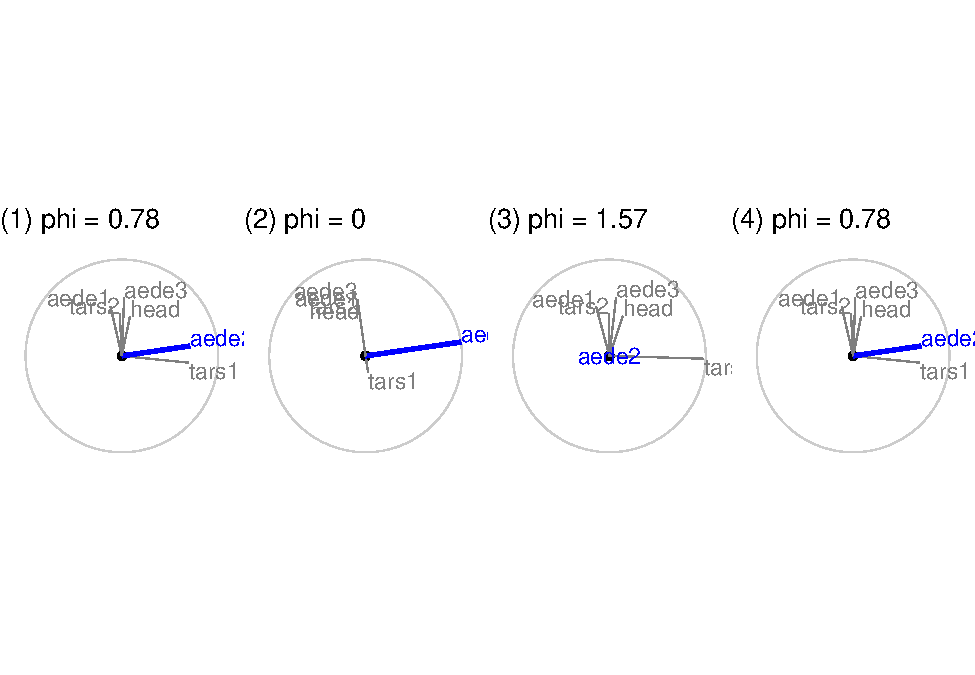
\includegraphics[width=1\linewidth]{spyrison-cook_files/figure-latex/step3-1} 

}

\caption[Snapshots of a radial manual tour manipulating aede2]{Snapshots of a radial manual tour manipulating aede2: (1) original projection, (2) full contribution, (3) zero contribution, (4) back to original. }\label{fig:step3}
\end{figure}
\end{Schunk}

\begin{enumerate}
\def\labelenumi{\arabic{enumi}.}
\tightlist
\item
  Set initial value of \(\phi_1\) and \(\theta\):
  \(\phi_1 = \cos^{-1}{\sqrt{B_{k1}^2+B_{k2}^2}}\),
  \(\theta = \tan^{-1}\frac{B_{k2}}{B_{k1}}\). Where \(\phi_1\) is the
  angle between \(\textbf{e}\) and its shadow in \(\textbf{B}\).
\item
  Set an angle increment (\(\Delta_\phi\)) that sets the step size for
  the animation, to rotate the manip var into and out of the projection.
  (Note: Using angle increment, rather than a number of steps, to
  control the movement, is consistent with the tour algorithm as
  implemented in the \pkg{tourr}).
\item
  Step towards \(0\), where the manip var is completely in the
  projection plane.
\item
  Step towards \(\pi/2\), where the manip variable has no contribution
  to the projection.
\item
  Step back to \(\phi_1\).
\end{enumerate}

In each of the steps 3-5, a small step may be added to ensure that the
endpoints of \(\phi\) (\(0\), \(\pi/2\), \(\phi_1\)) are reached.

\hypertarget{sec:display}{%
\subsubsection{Step 5) Projecting the data}\label{sec:display}}

The operation of a manual tour is defined on the projection bases. Only
when the data plot needs to be made is the data projected into the
relevant basis.

\begin{align*}
  \textbf{Y}^{(i)}_{[n,~3]} &= \textbf{X}_{[n,~p]} \textbf{M}_{[p,~3]} \textbf{R}^{(i)}_{[3,3]}
\end{align*}

\noindent where \(\textbf{R}^{(i)}_{[3,3]}\) is the incremental rotation
matrix, using \(\phi_i\). To make the data plot, use the first two
columns of \textbf{Y}. Show the projected data for each frame in
sequence to form an animation.

Figure \ref{fig:step4} illustrates a manual tour sequence having 15
steps. The projection axes are displayed on the top half, which
corresponds to the projected data in the bottom half. When aede2 is
removed from the projection, the purple cluster overlaps with the green
cluster. This suggests that aede2 is important for distinguishing
between these species.

Tours are typically viewed as an animation. The animation of this tour
can be viewed online at
\url{https://nspyrison.netlify.com/thesis/flea_manualtour_mvar5/}. The
page may take a moment to load. Animations can be produced using the
function \code{play\_manual\_tour()}.

\begin{Schunk}
\begin{figure}

{\centering 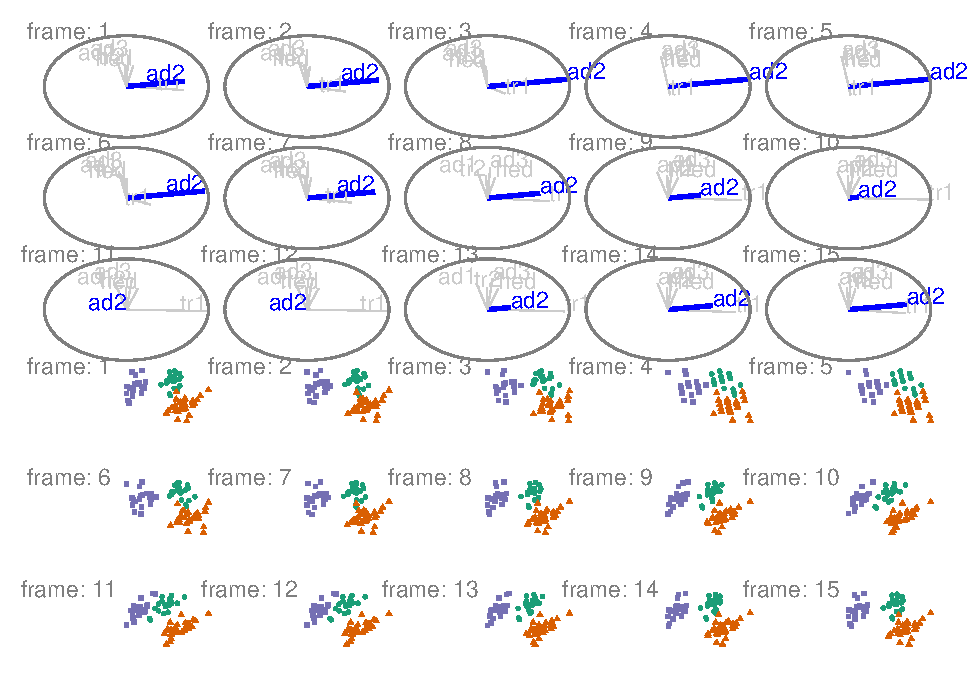
\includegraphics[width=5.83in,height=7in]{spyrison-cook_files/figure-latex/step4-1} 

}

\caption[Radial manual tour manipulating aede2 of standardized flea data]{Radial manual tour manipulating aede2 of standardized flea data. The axis for aede2 increases in contribution to the projection, from its initial value to 1, decreasing to 0 and then returning to the initial value. This effects the separation between the purple and green clusters. This shows that aede2 is important for distinguishing the purple species, because the separation disappears when aede2 is not contributing to the projection. An animation can be viewed at https://nspyrison.netlify.com/thesis/flea\_manualtour\_mvar5/.}\label{fig:step4}
\end{figure}
\end{Schunk}

\hypertarget{package-structure-and-functionality}{%
\section{Package structure and
functionality}\label{package-structure-and-functionality}}

This section describes the functions available in the package, and how
to use them.

\hypertarget{installation}{%
\subsection{Installation}\label{installation}}

The \pkg{spinifex} is available from CRAN, and can be installed by:

\begin{Schunk}
\begin{Sinput}
## Install from CRAN
install.package("spinifex")
## Load into session
library("spinifex")
\end{Sinput}
\end{Schunk}

\noindent Also see the shiny app for understandign and the vignette for
basic usage:

\begin{Schunk}
\begin{Sinput}
## Shiny app for visualizing basic application
run_app("intro")
## View the code vignette
vignette("spinifex_vignette")
\end{Sinput}
\end{Schunk}

\noindent The development version can be installed from github:

\begin{Schunk}
\begin{Sinput}
## Optionally install latest developmention version from GitHub
remotes::install_github("nspyrison/spinifex")
\end{Sinput}
\end{Schunk}

\hypertarget{functions}{%
\subsection{Functions}\label{functions}}

Table \ref{tab:functionsTable} lists the primary functions and their
purpose. These are grouped into four types: construction for building a
tour path, render to make the plot objects, animation for running the
animation, and specialty for providing illustrations used in the
algorithm description.

\begin{Schunk}
\begin{table}

\caption{\label{tab:functionsTable}Summary of available functions.}
\centering
\begin{tabular}[t]{lll}
\toprule
Type & Function & Description\\
\midrule
construction & create\_manip\_space & forms the 3D space of rotation\\
construction & rotate\_manip\_space & performs 3D rotation\\
construction & manual\_tour & generates sequence of 2D frames\\
 &  & \\
render & array2df & turn the tour path array into long form, for plotting\\
render & render\_ & render long form as a ggplot2 objection for animation\\
render & render\_plotly & render the animation as a plotly object (default)\\
render & render\_gganimate & render the animation as a gganimate object\\
 &  & \\
animation & play\_tour\_path & composite function animating the specified tour path\\
animation & play\_manual\_tour & composite function animating the specified manual tour\\
 &  & \\
specialty & oblique\_basis & table of the rotated basis and manip space\\
specialty & oblique\_frame & display the reference axes of a given basis\\
specialty & view\_manip\_space & illustrative display of any manip space\\
\bottomrule
\end{tabular}
\end{table}

\end{Schunk}

\hypertarget{sec:usage}{%
\subsection{Usage}\label{sec:usage}}

Using the \code{flea} data from the \pkg{tourr} package, we will
illustrate generating a manual tour to explore the sensitivity of the
cluster structure is to the variable aede2.

\begin{Schunk}
\begin{Sinput}
library(spinifex)
## Standardized flea data
f_data <- tourr::rescale(flea[, 1:6])
## Guided tour path, holes index
f_path <- save_history(f_data, guided_tour(holes()))
## Local extrema found
f_basis <- matrix(f_path[,, max(dim(f_path)[3])], ncol=2)
## Categorical class variable
f_cat <- factor(flea$species)
## Manip var, number of the variable to alter
f_mvar <- 5
## Anglular dist between frames (radians)
step_size <- .26
## Render and play animate, as plotly object by default
play_manual_tour(data = f_data,
                 basis = f_basis,
                 manip_var = f_mvar, 
                 angle = step_size,
                 col = f_cat,
                 pch = f_cat)
\end{Sinput}
\end{Schunk}

\noindent The \code{play\_manual\_tour()} function is a composite
function handling interaction between \code{manual\_tour()},
\code{array2df()}, and \code{render\_plotly()}. This will generate an
html animation using plotly. Switching the renderer to
\code{render\_gganimate()} alternatively creates an animated gif. Each
of these formats allows for the animation to be made available on a web
site, or directly visible in an html formatted document.

\hypertarget{making-illustrations}{%
\subsubsection{Making illustrations}\label{making-illustrations}}

The function \texttt{oblique\_frame} can be used to show a projection of
the basis, or with the data overlaid. For example, the plots in Figures
\ref{fig:step0} and \ref{fig:step3} were made with code similar to this:

\begin{Schunk}
\begin{Sinput}
## View a basis and projected data 
oblique_frame(basis = f_basis, 
              data = f_data,
              color = f_cat,
              shape = f_cat)
\end{Sinput}
\end{Schunk}

\noindent An illustration of the manip space (as shown in Figure
\ref{fig:step2}) is made with the \texttt{view\_manip\_space} function,
as follows:

\begin{Schunk}
\begin{Sinput}
## Displays the projection plane and manipulation space for the 
view_manip_space(basis = f_basis, 
                 manip_var = f_mvar, 
                 lab = colnames(f_data))
\end{Sinput}
\end{Schunk}

\hypertarget{sec:application}{%
\section{Application}\label{sec:application}}

\citet{wang_mapping_2018} introduces a new tool, PDFSense, to visualize
the sensitivity of hadronic experiments to nucleon structure. The
parameter-space of these experiments lies in 56 dimensions,
\(\delta \in \mathbb{R}^{56}\), and are visualized as 3D subspaces of
the 10 first principal components in linear (PCA) and non-linear (t-SNE)
embeddings.

\citet{cook_dynamical_2018} illustrates how to learn more about the
structures using a grand tour. Tours can better resolve the shape of
clusters, intra-cluster detail, and better outlier detection than
PDFSense \& TFEP (TensorFlow embedded projections) or traditional static
embeddings. This example builds from here, illustrating how the manual
tour can be used to examine the sensitivity of structure in a projection
to different parameters. The specific 2D projections passed to the
manual tour were provided in their work.

The data has a hierarchical structure with top-level clusters; DIS, VBP,
and jet. Each cluster is a particular class of experiments, each with
many experimental datasets which, each have many observations of their
own. In consideration of data density, we conduct manual tours on
subsets of the DIS and jet clusters. This explores the sensitivity of
the structure to each of the variables in turn and we present the
subjectively best and worst variable to manipulate for identifying
dimensionality of the clusters and describing the span of the clusters.

\hypertarget{jet-cluster}{%
\subsection{Jet cluster}\label{jet-cluster}}

The jet cluster resides in a smaller dimensionality than the full set of
experiments with four principal components explaining 95\% of the
variation in the cluster \citep{cook_dynamical_2018}. The data within
this 4D embedding is further subsetted, to ATLAS7old and ATLAS7new, to
focus on two groups that occupy different parts of the subspace. Radial
manual tours controlling contributions from PC4 and PC3 are shown in
Figures \ref{fig:JetClusterGood} and \ref{fig:JetClusterBad},
respectively. The difference in shape can be interpreted as the
experiments probing different phase-spaces. Back-transforming the
principal components to the original variables can be done for a more
detailed interpretation.

When PC4 is removed from the projection (Figure
\ref{fig:JetClusterGood}) the difference between the two groups is
removed, indicating that it is important for distinguishing experiments.
However, removing PC3 from the projection (Figure
\ref{fig:JetClusterBad}) does not affect the structure, indicating it is
not important for distinguishing experiments. Animations for the
remaining PCs can be viewed at the following links:
\href{https://nspyrison.netlify.com/thesis/jetcluster_manualtour_pc1/}{PC1},
\href{https://nspyrison.netlify.com/thesis/jetcluster_manualtour_pc2/}{PC2},
\href{https://nspyrison.netlify.com/thesis/jetcluster_manualtour_pc3/}{PC3},
and
\href{https://nspyrison.netlify.com/thesis/jetcluster_manualtour_pc4/}{PC4}.
It can be seen that only PC4 is important for viewing the difference in
these two experiments.

\begin{Schunk}
\begin{figure}

{\centering 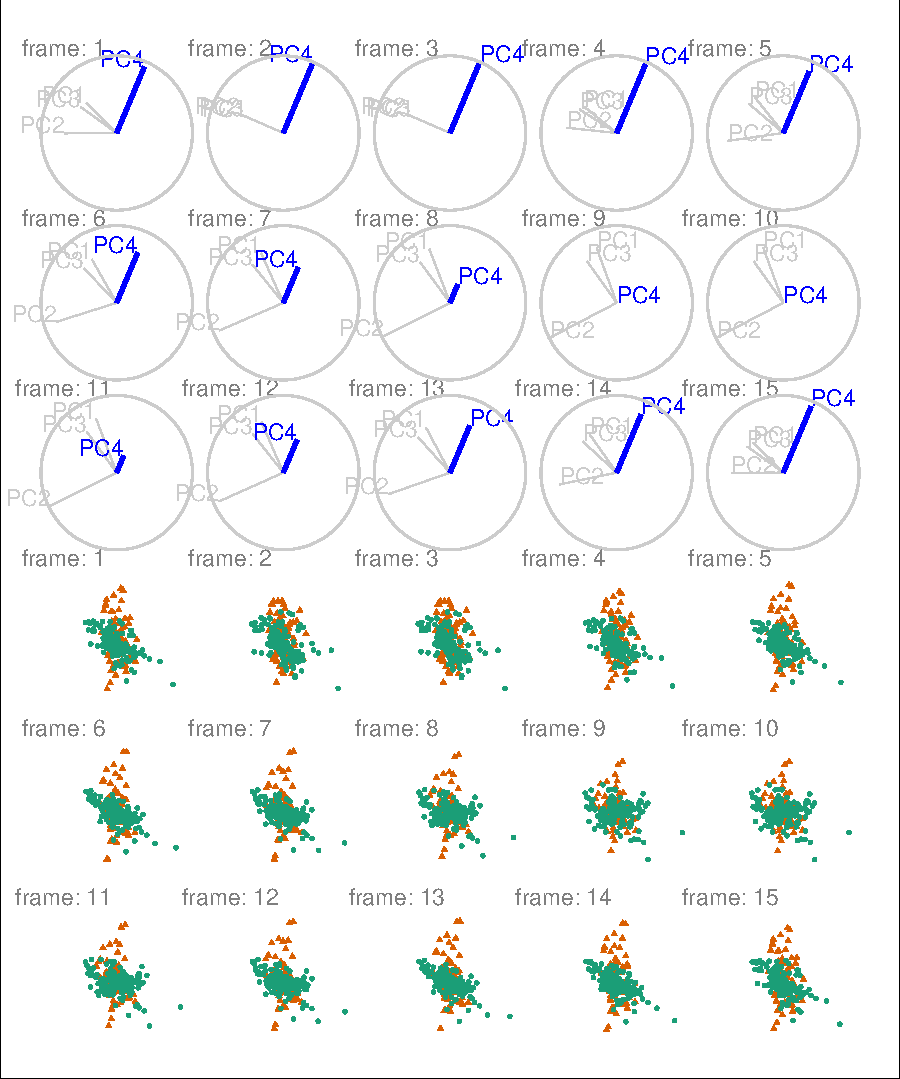
\includegraphics[width=5.83in,height=7in]{spyrison-cook_files/figure-latex/JetClusterGood-1} 

}

\caption[Snapshots of a radial manual tour of PC4 within the jet cluster, with color indicating experiment type]{Snapshots of a radial manual tour of PC4 within the jet cluster, with color indicating experiment type: ATLAS7new (green) and ATLAS7old (orange). When PC4 is removed from the projection (frame 10) there is little difference between the groups, suggesting that PC4 is important for distinguishing the experiments. The animation can be viewed at https://nspyrison.netlify.com/thesis/jetcluster\_manualtour\_pc4/.}\label{fig:JetClusterGood}
\end{figure}
\end{Schunk}

\begin{Schunk}
\begin{figure}

{\centering 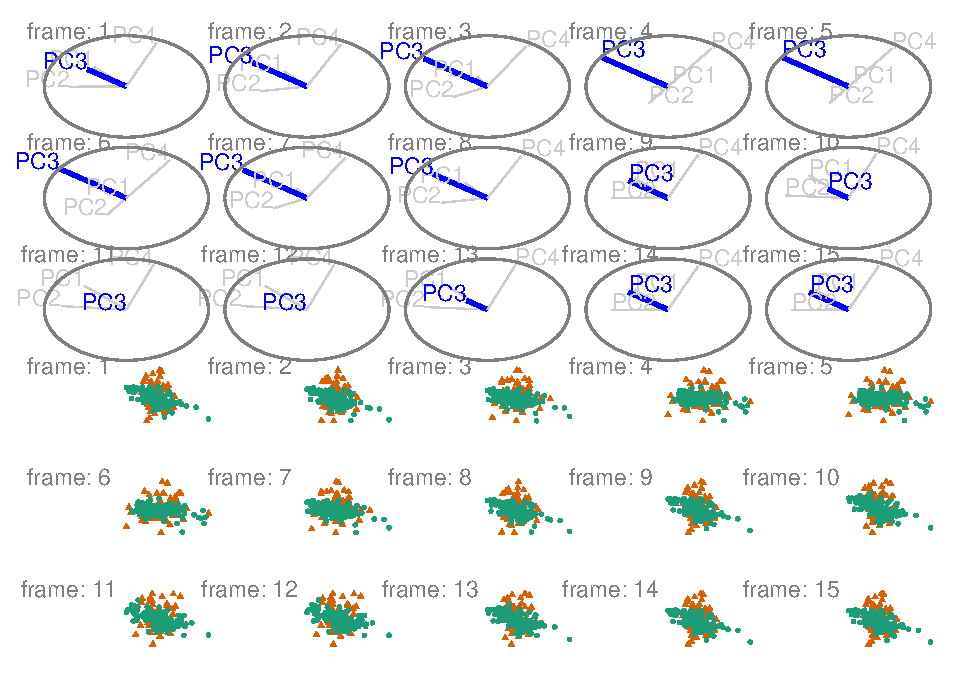
\includegraphics[width=5.83in,height=7in]{spyrison-cook_files/figure-latex/JetClusterBad-1} 

}

\caption[Snapshots of a radial manual tour of PC3 within the jet cluster, with color indicating experiment type]{Snapshots of a radial manual tour of PC3 within the jet cluster, with color indicating experiment type: ATLAS7new (green) and ATLAS7old (orange).  When the contribution from PC3 is changed there is little change to the structure of the two groups, suggesting that PC3 is not important for distinguishing the experiments. The animation can be viewed at https://nspyrison.netlify.com/thesis/jetcluster\_manualtour\_pc3/.}\label{fig:JetClusterBad}
\end{figure}
\end{Schunk}

\hypertarget{dis-cluster}{%
\subsection{DIS cluster}\label{dis-cluster}}

Following \citet{cook_dynamical_2018}, to explore the DIS cluster, PCA
is recomputed and the first six principal components, explaining 48\% of
the full sample variation, are used. The contributions of PC6 and PC2
are explored in Figures \ref{fig:DISclusterGood} and
\ref{fig:DISclusterBad}, respectively. Three experiments are examined:
DIS HERA1+2 (green), dimuon SIDIS (purple), and charm SIDIS (orange).

Both PC2 and PC6 contribute to the projection similarly. When PC6 is
rotated into the projection, variation in the DIS HERA1+2 is greatly
reduced. When PC2 is removed from the projection, dimuon SIDIS becomes
more clearly distinct. Even though both variables contribute similarly
to the original projection, their contributions have quite different
effects on the structure of each cluster, and the distinction between
clusters. Animations of all of the principal components can be viewed
from the links:
\href{https://nspyrison.netlify.com/thesis/discluster_manualtour_pc1/}{PC1},
\href{https://nspyrison.netlify.com/thesis/discluster_manualtour_pc2/}{PC2},
\href{https://nspyrison.netlify.com/thesis/discluster_manualtour_pc3/}{PC3},
\href{https://nspyrison.netlify.com/thesis/discluster_manualtour_pc4/}{PC4},
\href{https://nspyrison.netlify.com/thesis/discluster_manualtour_pc5/}{PC5},
and
\href{https://nspyrison.netlify.com/thesis/discluster_manualtour_pc6/}{PC6}.

\begin{Schunk}
\begin{figure}

{\centering 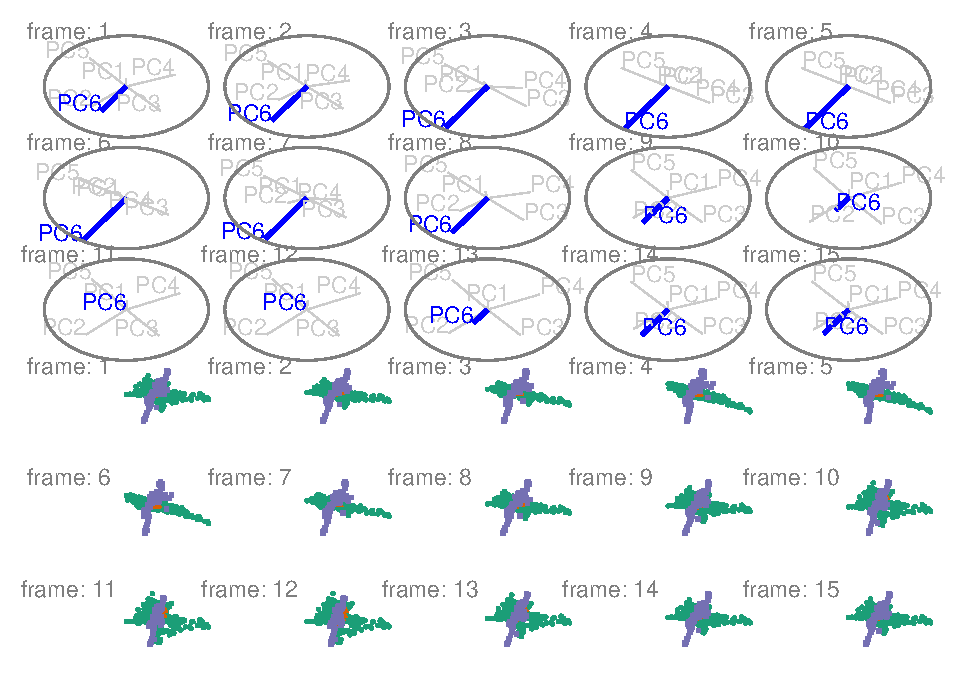
\includegraphics[width=5.83in,height=7in]{spyrison-cook_files/figure-latex/DISclusterGood-1} 

}

\caption[Snapshots of a radial manual tour exploring the sensitivity PC6 has on the structure of the DIS cluster, with color indicating experiment type]{Snapshots of a radial manual tour exploring the sensitivity PC6 has on the structure of the DIS cluster, with color indicating experiment type: DIS HERA1+2 (green), dimuon SIDIS (purple), and charm SIDIS (orange). DIS HERA1+2 is distributed in a cross-shaped plane, charm SIDIS occupies the center of this cross, and dimuon SIDIS is a linear cluster crossing DIS HERA1+2. As the contribution of PC6 is increased, DIS HERA1+2 becomes almost singular in one direction (frame 5), indicating that this experiment has very little variability in the direction of PC6. The animation can be viewed at https://nspyrison.netlify.com/thesis/discluster\_manualtour\_pc6/.}\label{fig:DISclusterGood}
\end{figure}
\end{Schunk}

\begin{Schunk}
\begin{figure}

{\centering 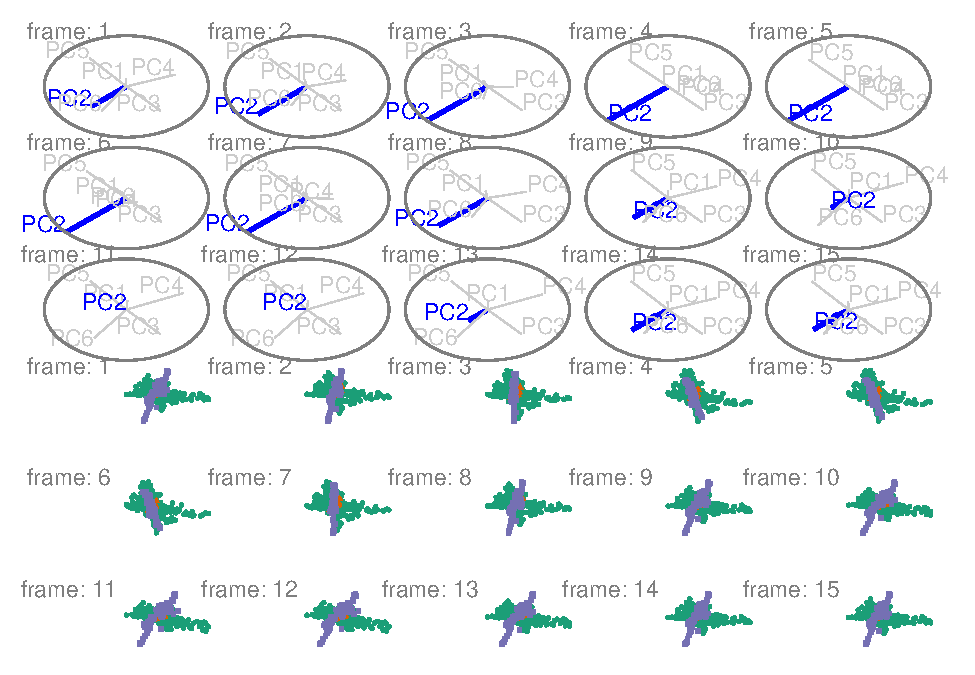
\includegraphics[width=5.83in,height=7in]{spyrison-cook_files/figure-latex/DISclusterBad-1} 

}

\caption[Snapshots of a radial manual tour exploring the sensitivity PC2 to the structure of the DIS cluster, with color indicating experiment type]{Snapshots of a radial manual tour exploring the sensitivity PC2 to the structure of the DIS cluster, with color indicating experiment type: DIS HERA1+2 (green), dimuon SIDIS (purple), and charm SIDIS (orange). As contribution from PC2 is decreased, dimuon SIDIS becomes more distinguishable from the other two clusters (frames 10-14), indicating that in its absence PC2 is important. The animation can be viewed at https://nspyrison.netlify.com/thesis/discluster\_manualtour\_pc2/.}\label{fig:DISclusterBad}
\end{figure}
\end{Schunk}

\hypertarget{sec:discussion}{%
\section{Discussion}\label{sec:discussion}}

Dynamic linear projections of numeric multivariate data, tours, play an
important role in data visualization; they extend the dimensionality of
visuals to peek into high-dimensional data and parameter spaces. This
research has taken the manual tour algorithm, specifically the radial
rotation, used in GGobi \citep{swayne_ggobi:_2003} to interactively
rotate a variable into or out of a 2D projection, and modified it to
create an animation that performs the same task. It is most useful for
examining the importance of variables, and how the structure in the
projection is sensitive or not to specific variables. This functionality
available in package \pkg{spinifex}. The work complements the methods
available in the \pkg{tourr} package.

This work was motivated by problems in physics, and thus the usage was
illustrated on data comparing experiments of hadronic collisions, to
explore the sensitivity of cluster structure to different principal
components. These tools can be applied quite broadly to many
multivariate data analysis problems.

The manual tour is constrained in the sense that the effect of one
variable is dependent on the contributions of other variables in the
manip space. However, this can be useful to simplify a projection by
removing variables without affecting the visible structure. Defining a
manual rotation in high dimensions is possible using Givens rotations
and Householder reflections as outlined in
\citet{buja_computational_2005}. This would provide more flexible manual
rotation, but more difficult for a user because they have the choice
(too much choice) of which directions to move.

Another future research topic could be to extend the algorithm for use
on 3D projections. With the current popularity and availability of 3D
virtual displays, this may benefit the detection and understanding of
the higher dimensional structure, or enable the examination of
functions.

Having a graphical user interface would be useful for making it easier
and more accessible to a general audience. This is possible to implement
using \CRANpkg{shiny} \citep{chang_shiny_2020}. The primary purposes of
the interface would be to allow the user to interactively change the
manip variable easily, and the interpolation step for more or less
detailed views.

\hypertarget{acknowledgments}{%
\section{Acknowledgments}\label{acknowledgments}}

This article was created in R, using \CRANpkg{knitr}
\citep{xie_knitr_2020} and \CRANpkg{rmarkdown}
\citep{allaire_rmarkdown_2020}, with code generating the examples
inline. The source files for this article be found at
\href{https://github.com/nspyrison/spinifex_paper/}{github.com/nspyrison/spinifex\_paper/}.
The source code for the \pkg{spinifex} package can be found at
\href{https://github.com/nspyrison/spinifex/}{github.com/nspyrison/spinifex/}.

\bibliography{spyrison-cook.bib}

\address{%
Nicholas Spyrison\\
Monash University\\
Faculty of Information Technology\\
}
\href{mailto:nicholas.spyrison@monash.edu}{\nolinkurl{nicholas.spyrison@monash.edu}}

\address{%
Dianne Cook\\
Monash University\\
Department of Econometrics and Business Statistics\\
}
\href{mailto:dicook@monash.edu}{\nolinkurl{dicook@monash.edu}}

